\chapter{MEASUREMENTS OF ATOM VELOCITY USING PHASE CHOPPERS}
\label{choppersChapter}

Section \ref{choppersBrief}, Appendix B and C.E. Klauss' B.S.~thesis \cite{Kla11} discuss our use of phase choppers to measure atom beam velocity. Section \ref{polChapterGradElg} shows polarizability measurements obtained after measuring atom beam velocity using phase choppers. Here, we provide samples of the pictures used to determine the distance between the phase choppers. I also discuss the ability of phase choppers to act as lenses for atomic de Broglie waves.




%%%%%%%%%%%%%%%%%%%%%%%%%%%%%%%%%%%%%%%%%%%%%%
\section{Distance measurements using high resolution pictures}
\label{distMeasurements}
The accuracy of the velocity measurement using phase choppers can only be as good as the measurement of the distance between the two choppers. To measure this distance (and others in the machine) we carefully inserted a series of rulers and tape measures into the vacuum chamber and took high resolution pictures of the choppers next to the measuring devices, such as the ones shown in Figure \ref{distMeas_c1e_c2w} and Figure \ref{distMeas_2g}. We mounted the camera (a Canon PowerShot S90) on a translation stage to accurately center the high-voltage wire in the middle of the frame and avoid angular misalignments. This minimized errors due to distortion and parallax. We then used optical and digital zoom to determine the positions of the choppers with respect to the tape measures with 100 $\mu$m precision. We used additional rulers and calipers to calibrate the accuracy of the tape measure.


We also took additional pictures with a vertically oriented ruler to determine the height at which the atom beam crosses the phase choppers, as well the angle of the choppers with respect to vertical by placing a plumb line next to the choppers. An example of the plumb line is shown in Figure \ref{distMeas_c1e_c2w}. These two measurements are combined to measure the distance between the two choppers where it counts: at the height of the atom beam. 


\begin{figure}
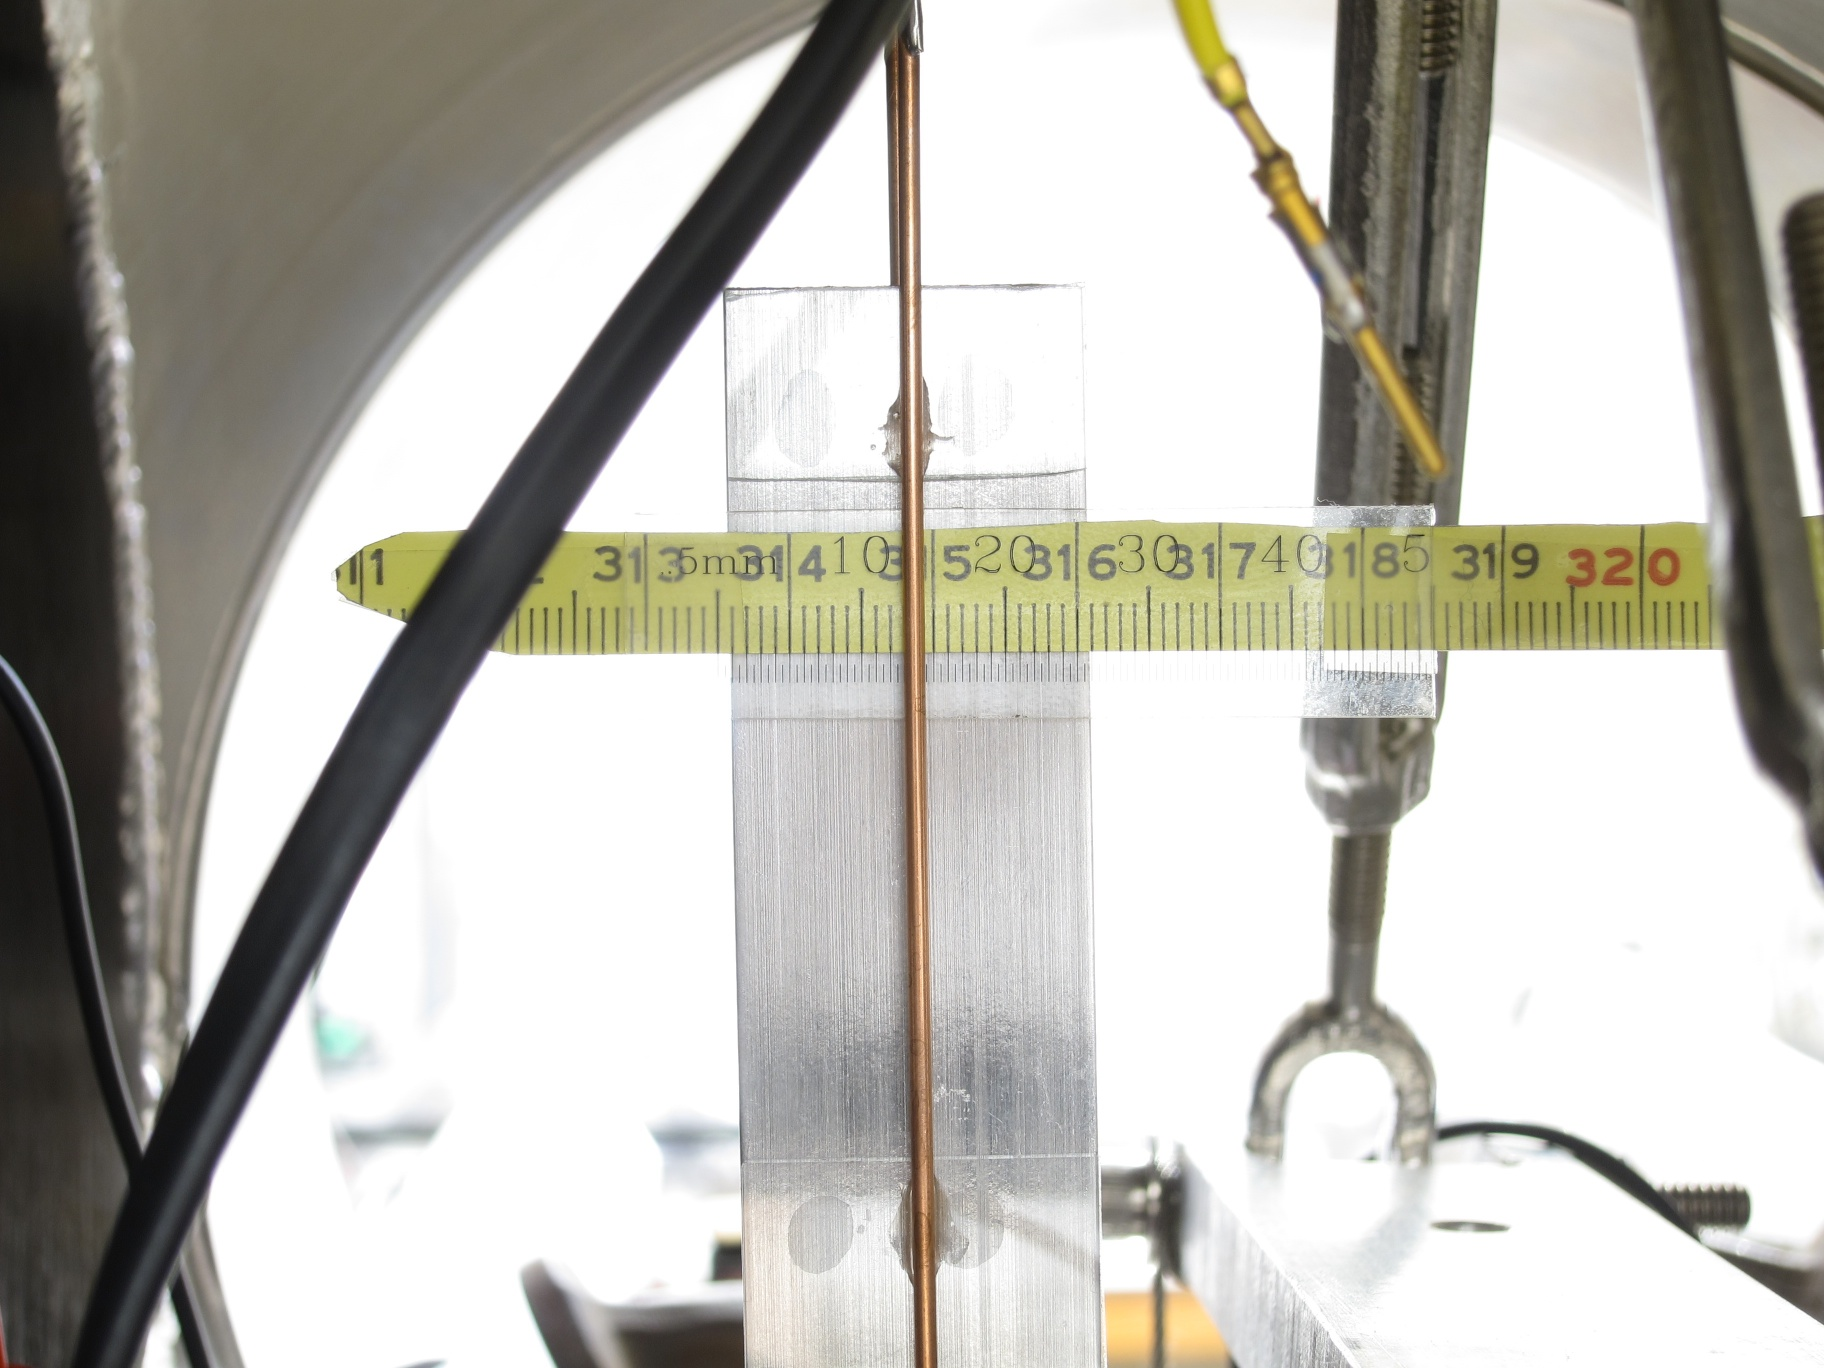
\includegraphics[width=0.5\textwidth]{Figures/distMeas_c1e.jpg}
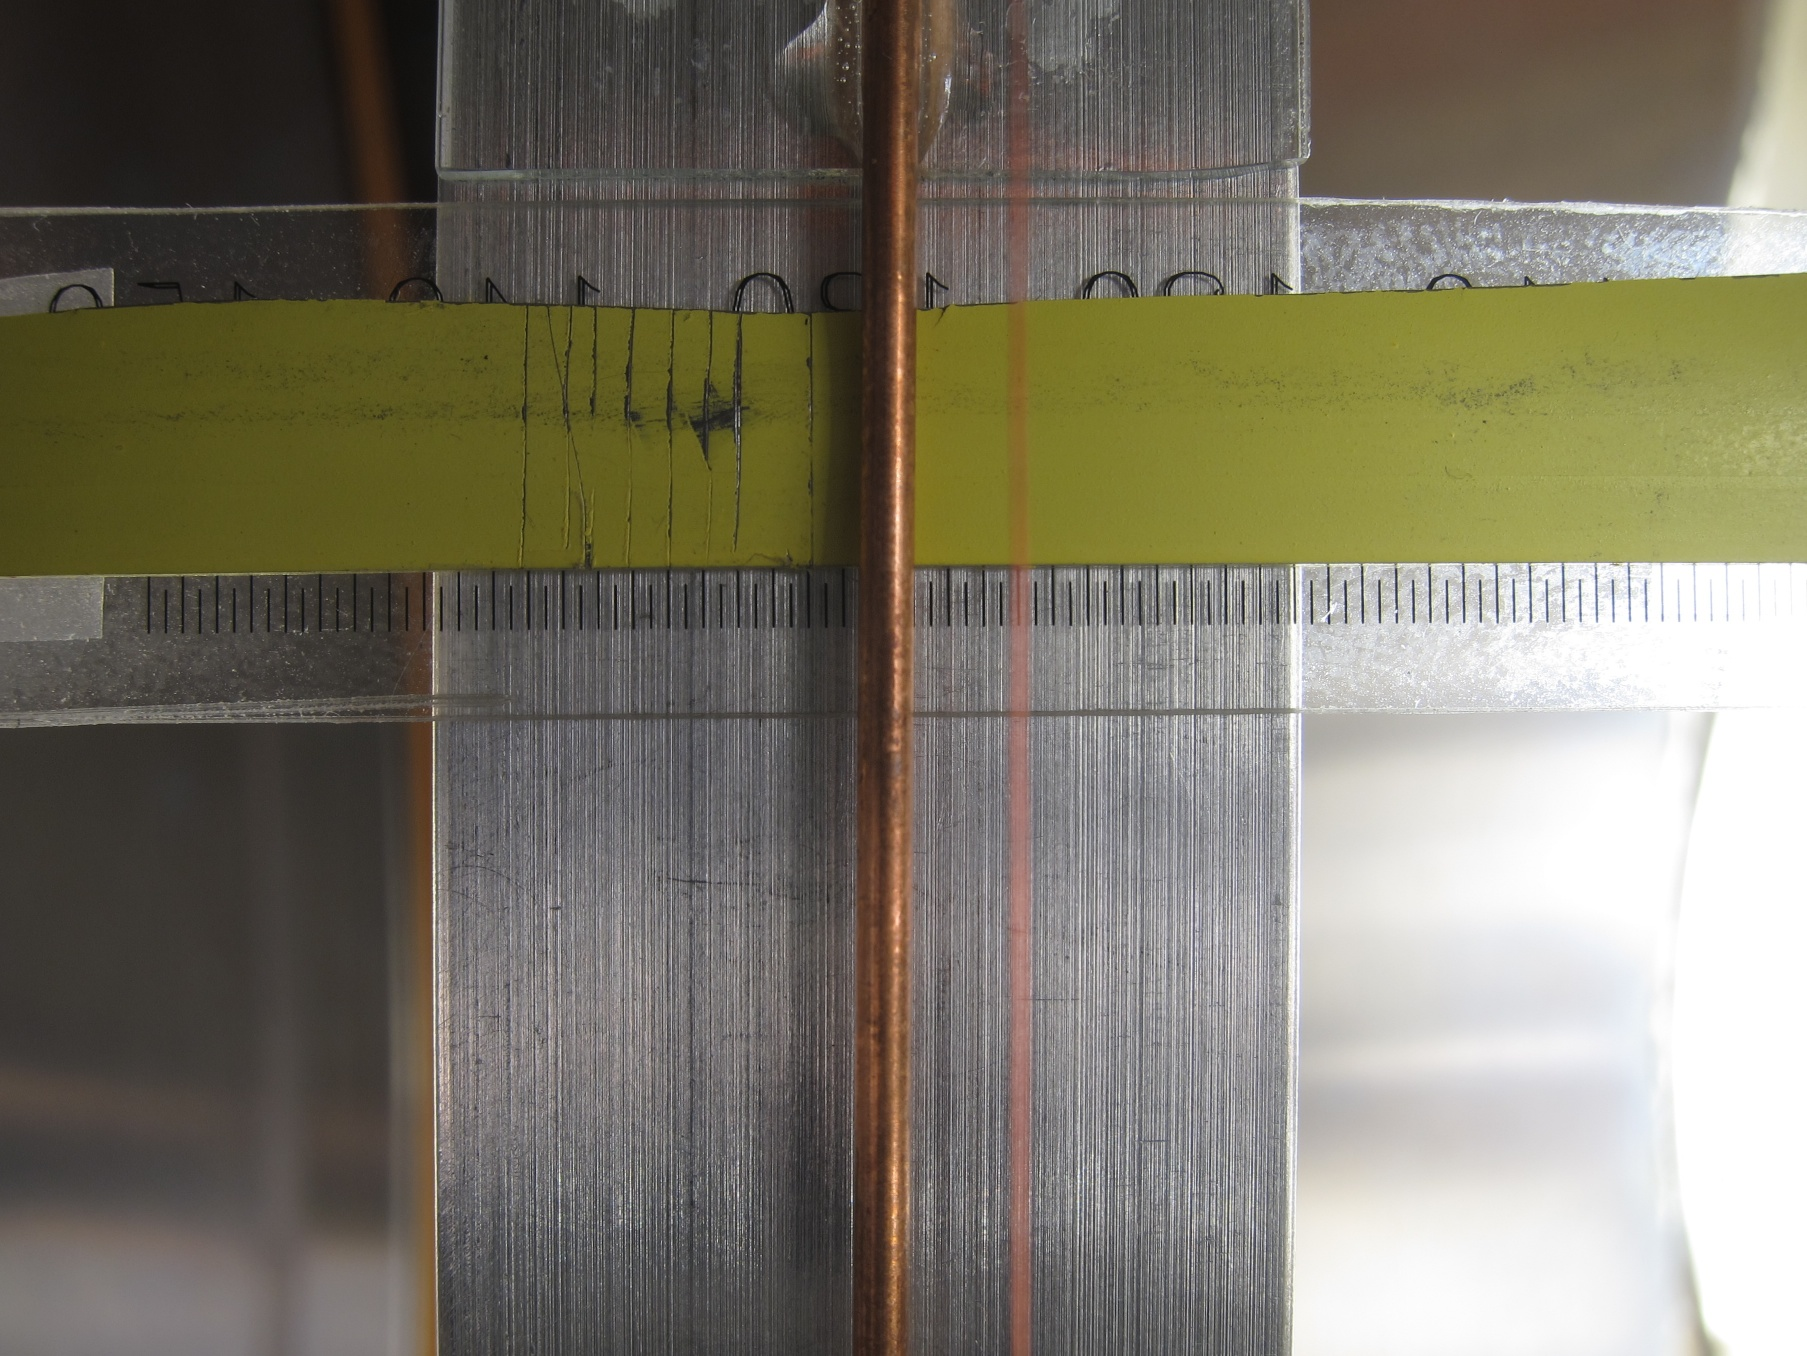
\includegraphics[width=0.5\textwidth]{Figures/distMeas_c2w.jpg}
\caption[Photographs for the measurement of the distance between chopper 1 and chopper 2.]{\label{distMeas_c1e_c2w}Measurement of the distance between chopper 1 and chopper 2 using a tape measure strung through the vacuum chamber above the atom beam path. Chopper 1 east side (left), and chopper 2 west side (right) are pictured. A transparent ruler serves as a translator between the two sides of the tape measure. The total uncertainty of this distance measurement is 250 $\mu$m. A plumb line (red) next to chopper 2 is also shown. Figure \ref{distMeas_2g} shows the approximate midpoint of the ruler above the 2nd nanograting.}
\end{figure}


\begin{figure}
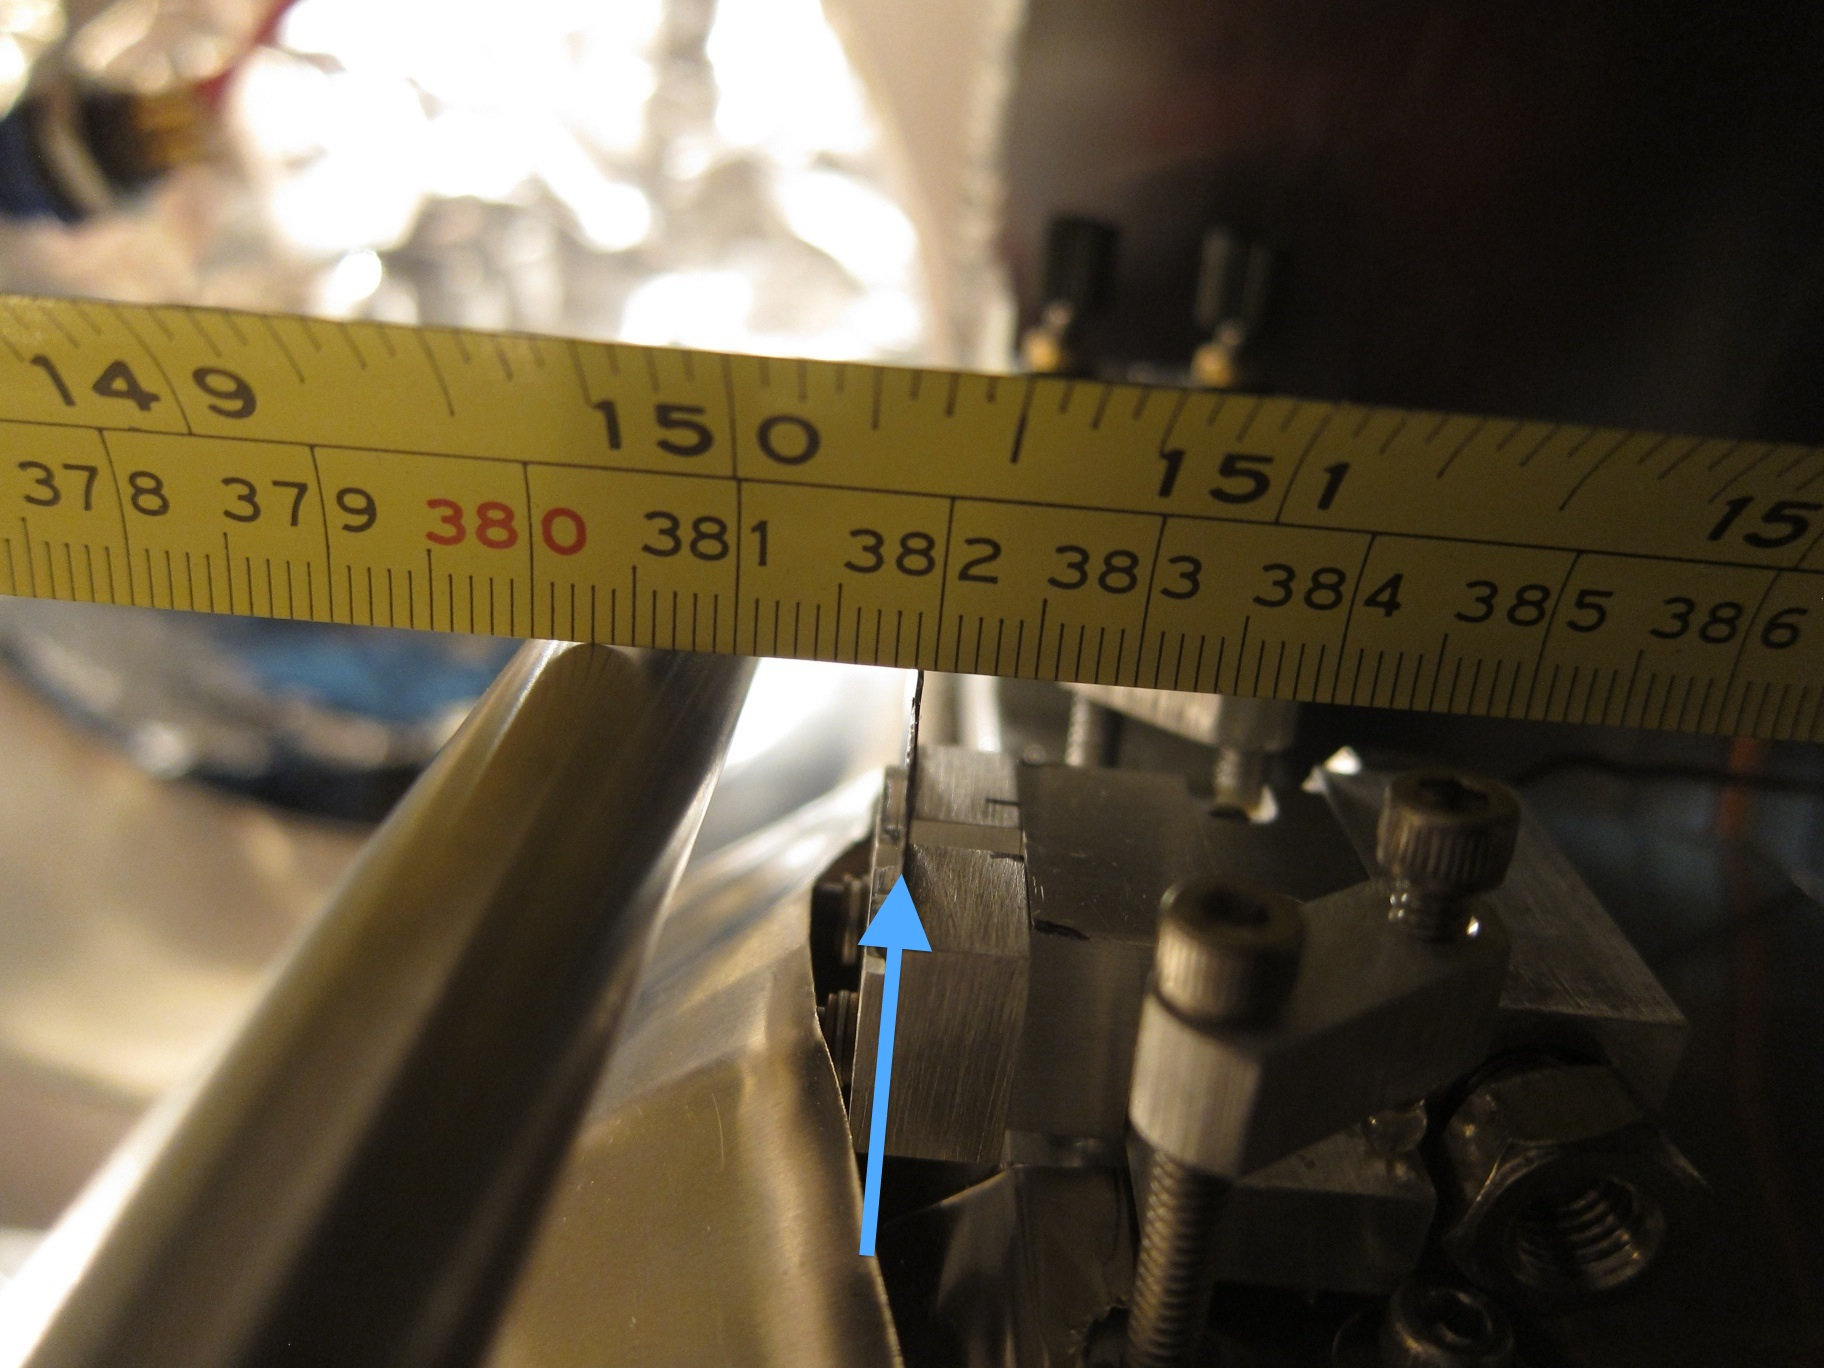
\includegraphics[width=1\textwidth]{Figures/distMeas_2g_arrow.jpg}
\caption[Photograph for the measurement of the distance between chopper 1 and chopper 2 showing the 2nd nanograting.]{\label{distMeas_2g}Measurement of the distance between chopper 1 and chopper 2. Two different nanogratings (both suitable for use as the second nanograting in the interferometer) are viewed edge-on and highlighted with a blue arrow. This allows us to determine the position of the 2nd grating with respect to the two phase choppers.}
\end{figure}





%%%%%%%%%%%%%%%%%%%%%%%%%%%%%%%%%%%%%%%%%%%%%%
\section{An electrostatic lens for matter waves inside an atom interferometer}
\label{lensSection}
In trying to reconcile small but persistent differences between the expected and observed interferometer contrast when using phase choppers, we discovered that our phase choppers can act as a lens for matter waves in our atom interferometer. Phase choppers, like all of the interaction regions described in this thesis, apply phase shifts that are a function of atom beam velocity. We would therefore naively assume that this dispersive phase shift would lead to a decrease in the measured contrast due to the velocity distribution of the atom beam. Instead, we observed that chopper 2 could \emph{increase} the interferometer contrast. Figure \ref{c2dcIncrease} shows an example of the interferometer contrast increasing when chopper 2 applies a differential phase shift. 


The key to understanding this effect is to realize that we detect the fringes formed by two complementary interferometers (formed by the +1, 0, and -1 diffraction orders from the first nanograting) and that the fringes formed by the two interferometers will not have the same phase unless the distance between the first and second nanogratings is exactly equal to the distance between the second and third nanograting. That is, if $d_\textrm{1G2G} \neq d_\textrm{2G3G}$ there will be a phase mismatch between the two interferometers, and thus a loss of contrast. Figure \ref{lens2IFM} shows a two interferometer model with chopper 1, the polarizability pillars, and chopper 2. Any of these electrodes can in principle correct for a phase mismatch between the two interferometers, provided that the sign of the phase shift is correct and the contrast loss due to the velocity distribution is negligible. However, chopper 2 can more easily correct the phase mismatch because of the larger spatial separation between the two interferometers at its location. This process is analogous to a diverging lens for matter waves in the atom interferometer acting to magnify the atom interference fringes. The consequences of this mechanism will be detailed in a future publication from our group.


Our \emph{New Journal of Physics} paper \cite{Hol11}, included in Appendix B, acknowledges that we could not explain the small difference between the measured reference contrast and the best-fit contrast determined using $\chi^2$ minimization. This problem was largely irrelevant to the determination of the atom beam velocity because it does not directly effect the frequencies at which the contrast revivals and minima occur. The contrast discrepancies do, however, effect the determination of the width of the velocity distribution. This in turn slightly changes the best estimate of the average velocity. In Holmgren \etal \cite{Hol11}, we estimated a 0.04\% systematic error in velocity may be present due to this discrepancy. We now understand that the magnitude of the error depends on the distance mismatch between the three nanogratings and may be several times larger unless we take more care to align the interferometer. Clearly, the highest accuracy measurements of atom beam velocity demand a full understanding of the data, and we are developing a more sophisticated model to incorporate these lensing effects.


\begin{figure}
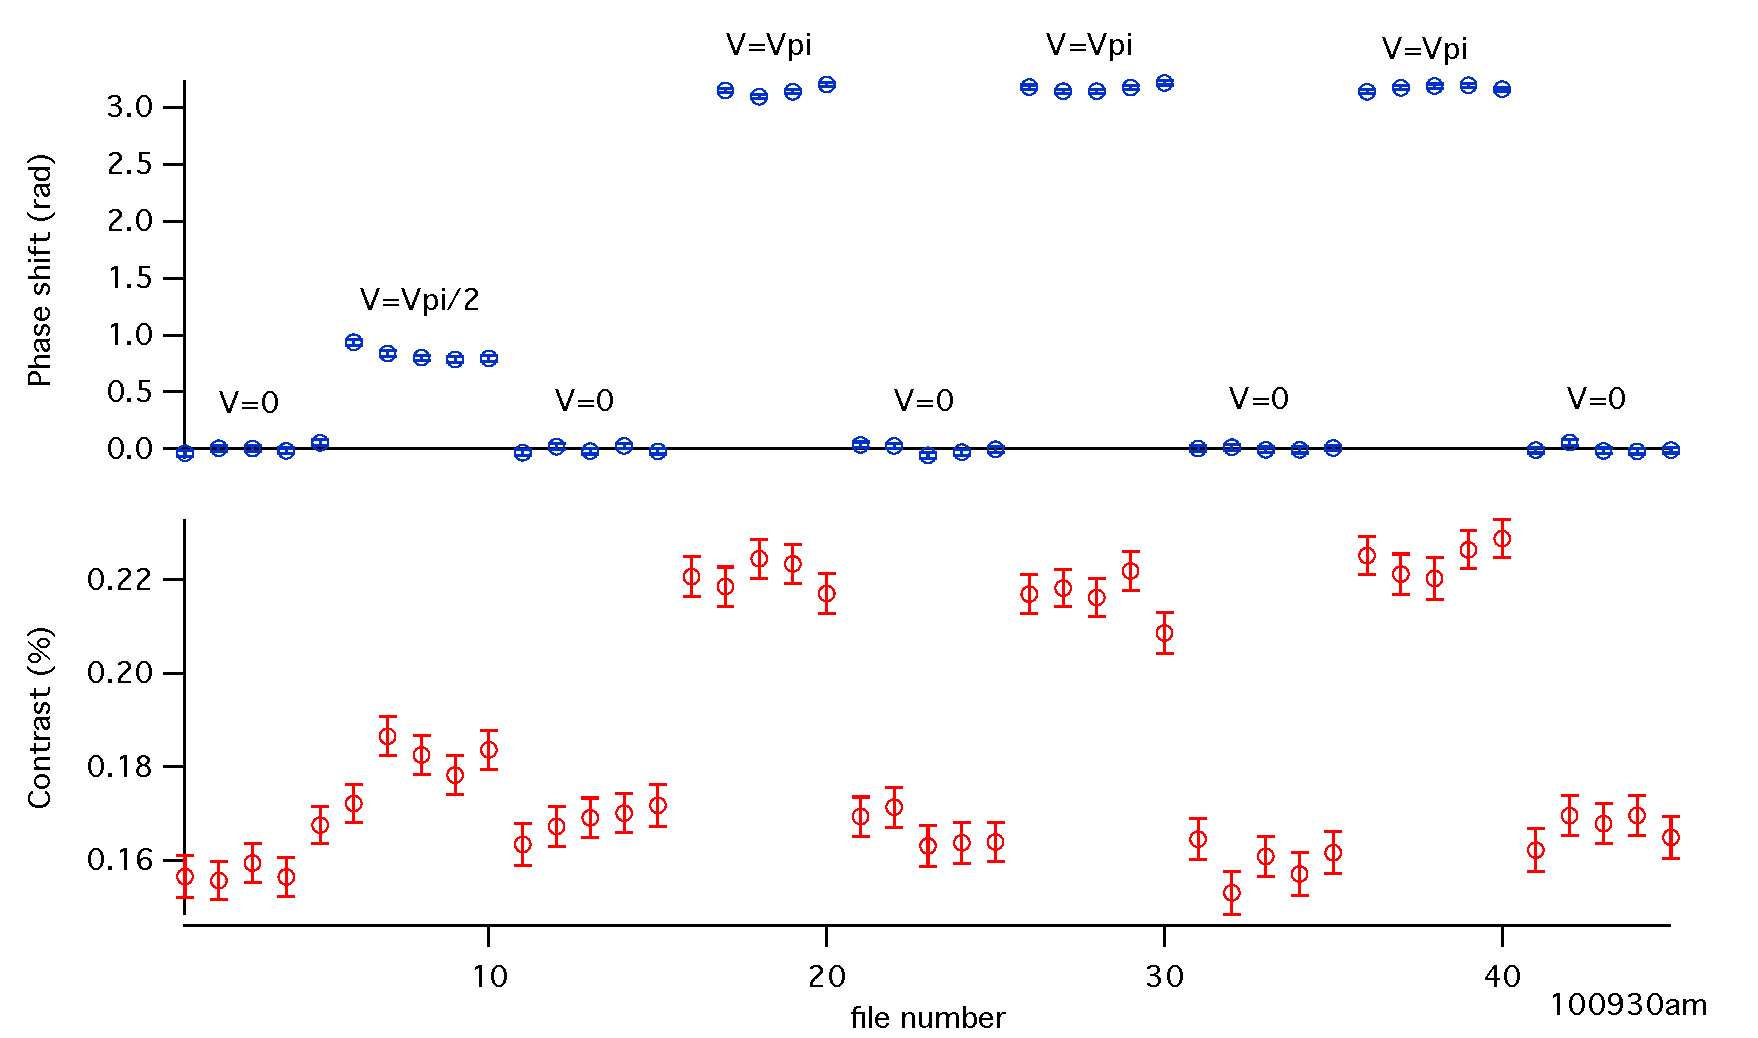
\includegraphics[width=1\textwidth]{Figures/contrastIncrease.pdf}
\caption[Unexpected increase in interferometer contrast due to energizing phase chopper 2.]{\label{c2dcIncrease}Interferometer phase shift (blue) and contrast (red) for three different voltages applied to chopper 2. $V_\pi$ is the voltage necessary to create a $\pi$ phase shift. The interferometer contrast \emph{increases} when a voltage is applied due to the \emph{rephasing}, or alternatively, the \emph{lensing} ability of chopper 2.}
\end{figure}


\begin{figure}
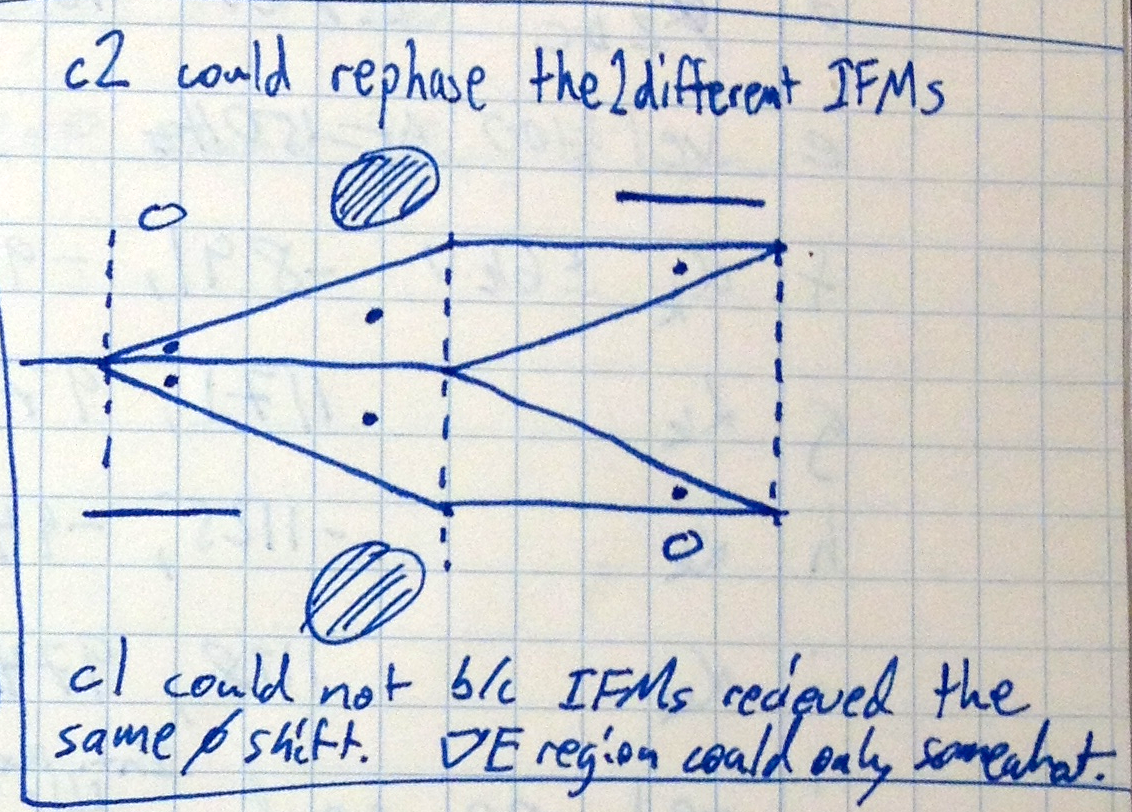
\includegraphics[width=1\textwidth]{Figures/lens2IFMnotebook.png}
\caption[Sketch of chopper 1, the polarizability electrodes, and chopper 2 with a two interferometer model.]{\label{lens2IFM}Nanogratings form multiple interferometers whose centerlines (marked with dots) diverge as a function of distance from the first nanograting. These two interferometers acquire different phase shifts because the electric field gradient is not uniform. The mismatch between interferometer phase shifts normally leads to a loss of observed contrast, but it can also lead to an increase in observed contrast if the distance between the first and second nanogratings is not equal to the distance between the second and third nanogratings. The phase choppers c1 and c2 are represented by small circles and thin lines (see Figure \ref{choppersIFMsimple}) and the polarizability interaction region is represented by slashed circles (see Figure \ref{IFMpillarsTrans}). Figure from page 31 of Tucson Book 13, October 5, 2011.}
\end{figure}




